\chapter{Vorgehen}
\label{chp:procedure}
In Kapitel \ref{chp:sequences} wurden Sequenzen, ihre Eigenschaften und die Möglichkeiten der Klassifizierung vorgestellt. Im Folgenden wird anhand eines fiktiven Beispiels das Vorgehen zur Wissensgenerierung aus Produktionsdaten - auf Grundlage der vorgenommenen Definitionen - beschrieben. Es werden die Daten von zwei Produktionsmaschinen, welche in einer Fertigungslinie hintereinander angeordnet sind (vgl. Abbildung \ref{fig:production-line}), miteinander verglichen.

\begin{figure}[H]
	\centering
	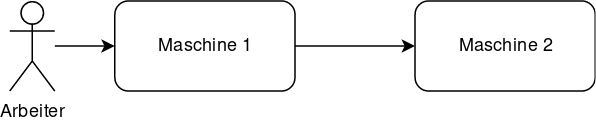
\includegraphics[scale=0.40]{images/Vorgehen/fertigungslinie}
	\caption{Fertigungslinie mit zwei Maschinen}
	\label{fig:production-line}
\end{figure}

In diesem Beispiel wird Maschine 1 mit Stückteilen befüllt. Diese werden dort vorverarbeitet und an Maschine 2 zur Endverarbeitung weitergegeben. Eine Produktionsmaschine kann laufen, warten oder stehen. Bei der Datenerhebung wird dabei zwischen vier möglichen Zuständen unterschieden (vgl. Tabelle \ref{tab:status-in-production}). 

\begin{table}
	\begin{center}
		\begin{tabular}{|c c c|} 
			\hline
			Symbol & Zustand & Beschreibung \\
			\hline\hline
			0 & läuft & Maschine läuft im Standardbetrieb \\ 
			\hline
			1 & steht & Maschine wurde durch Mitarbeiter angehalten \\
			\hline
			2 & steht & Maschine hat von alleine angehalten \\
			\hline
			3 & wartet & Maschine wartet auf Vorgänger in Fertigungslinie \\
			\hline
		\end{tabular}
		\caption{Zustände in Fertigungslinie}
		\label{tab:status-in-production}
	\end{center}
\end{table}

In diesem Beispiel werden die erhobenen Daten zum aktuellen Zustand der beiden Maschinen für einen Tag betrachtet. Dabei wird von 16 Arbeitsstunden und einer Datenerhebung pro Minute ausgegangen, weshalb für jede Maschine 960 Datenpunkte generiert werden (vgl. Abbildung \ref{fig:raw-data}).

\begin{figure}[H]
	\centering
	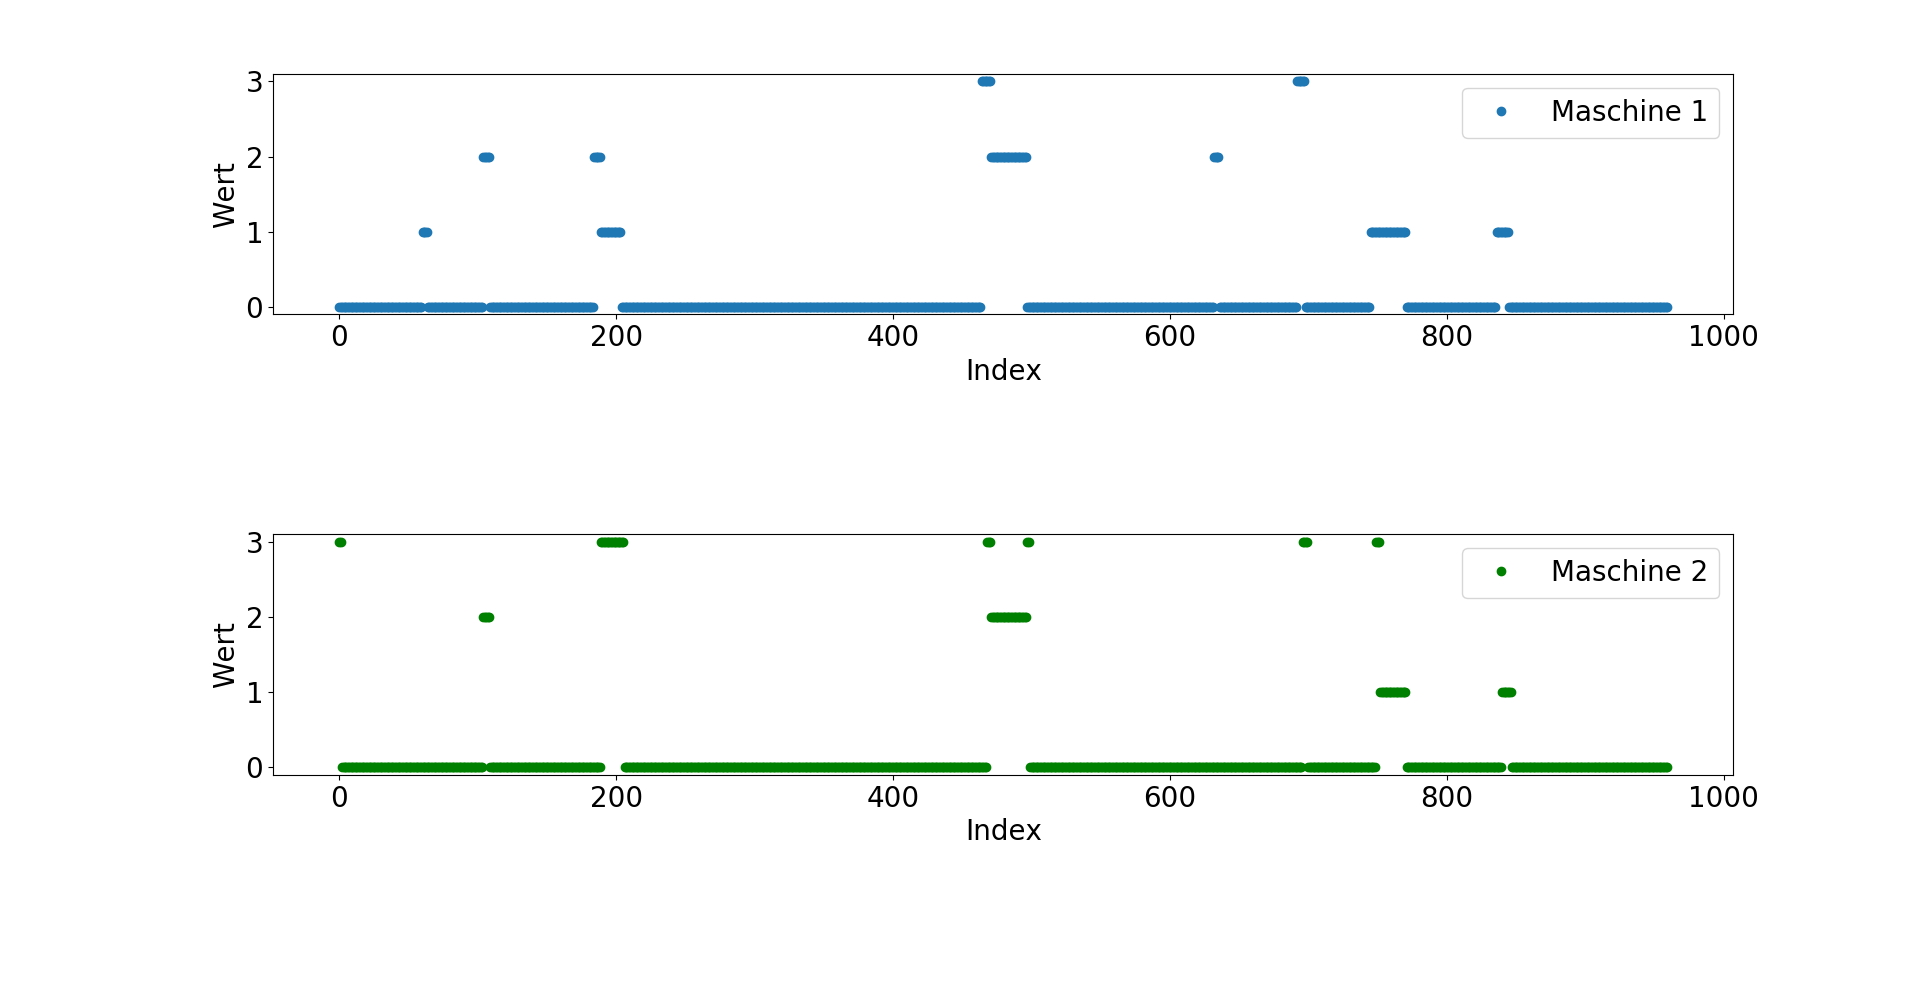
\includegraphics[scale=0.32]{images/Vorgehen/raw_data}
	\caption{Produktionsdaten Fertigungslinie (roh)}
	\label{fig:raw-data}
\end{figure}

\section{1. Datenaufbereitung}
Anders als bei simulierten Daten, muss man bei Produktionsdaten mit Fehlern rechnen. So kann es schon durch einen verdreckten Sensor zu Messfehlern oder Lücken in den Messreihen kommen\footnote{T.A. Runkler, Data Mining, Springer, 2015}. Fehler müssen somit entfernt oder korrigiert werden. Die im Folgenden beschriebenen Schritte haben daher zur Annahme, dass eine umfassende Aufbereitung der Daten vorgenommen wurde.

Als erstes werden die Produktionsdaten auf binäre Sequenzen reduziert. Dazu müssen die Zustände (Tabelle \ref{tab:status-in-production}) in die Kategorien \textit{Fehlerzustand} und \textit{kein Fehlerzustand} aufgeteilt werden. Zur ersten Kategorie gehören dabei die Zustände 1,2 und 3, da es sich bei diesen um ein unerwünschtes Verhalten im Sinne eines reibungslosen Produktionsprozesses handelt. Der einzige fehlerfreie Zustand bleibt die 0 (vgl. Tabelle \ref{tab:reduced-status-in-production}).

\begin{table}
	\begin{center}
		\begin{tabular}{|c c c|} 
			\hline
			Symbol & Zustand & Beschreibung \\
			\hline\hline
			0 & kein Fehlerzustand & Maschine läuft im Standardbetrieb \\ 
			\hline
			1 & Fehlerzustand & Maschine wartet oder wurde durch Mitarbeiter / von selbst angehalten  \\
			\hline
		\end{tabular}
		\caption{Reduzierte Zustände in Fertigungslinie}
		\label{tab:reduced-status-in-production}
	\end{center}
\end{table}

Bei diesem Arbeitsschritt zeigt sich, dass es bereits schwierig sein kann die ursprünglichen Zustände auf zwei zu reduzieren. In diesem Beispiel könnte der Zustand \textit{wartet} (Tabelle \ref{tab:status-in-production}) auch als \textit{kein Fehlerzustand} gewertet werden, da das Warten einer Maschine an sich kein Fehlverhalten ist. Hier wird er allerdings als \textit{Fehlerzustand} gewertet, da es in dieser Fertigungslinie Abhängigkeiten der Maschinen untereinander gibt. Daher kann bspw. das Warten von Maschine 2 auf einen Fehler von  Maschine 1 zurückgeführt werden.

Wenn man das Ergebnis der Datenaufbereitung visualisiert (Abbildung \ref{fig:reduced-data}), zeigt sich die gewünschte Vereinfachung auf zwei Zustände.

\begin{figure}[H]
	\centering
	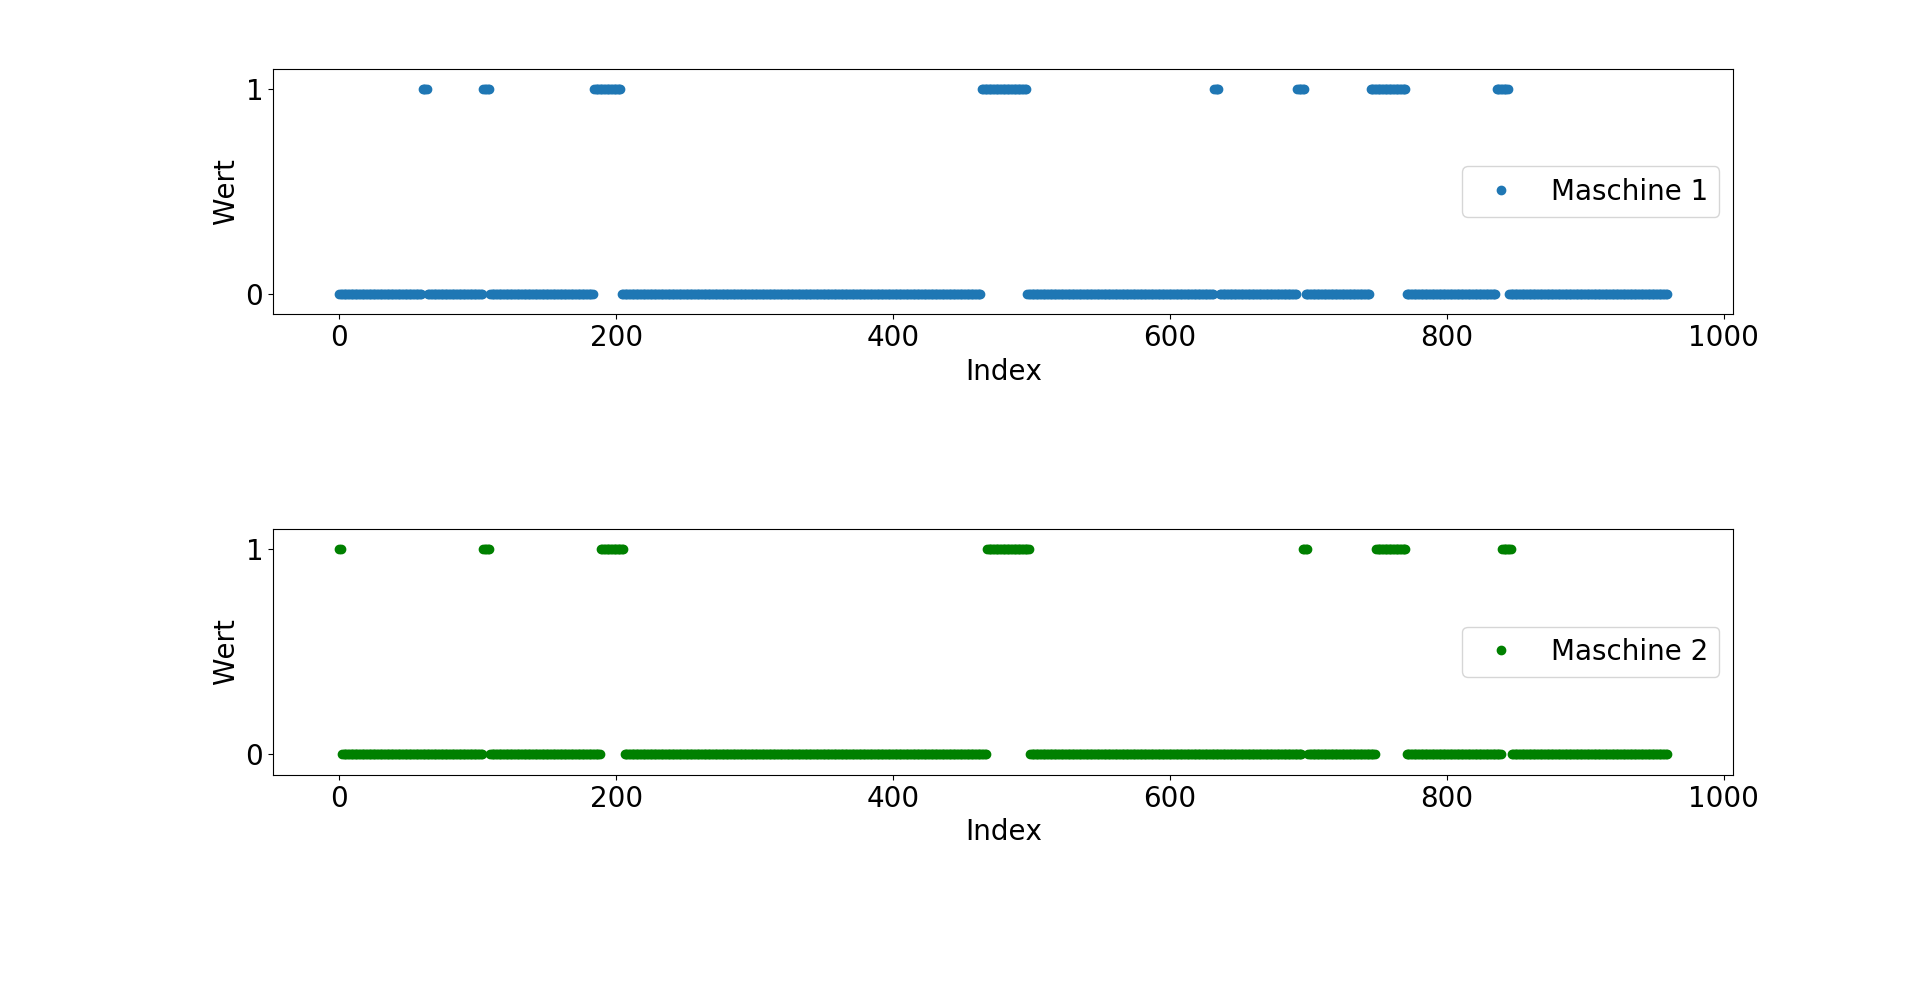
\includegraphics[scale=0.32]{images/Vorgehen/reduced_data}
	\caption{Produktionsdaten Fertigungslinie (reduziert)}
	\label{fig:reduced-data}
\end{figure}

\section{2. Klassifizierung}
Die Klassifizierung beginnt damit, dass die Balance und Frequenz für beide Sequenzen nach \ref{eq:balance} und \ref{eq:frequence} berechnet werden.
\begin{itemize}
	\item $Balance_{M1}(0) = 0.8885$ sowie $Balance_{M1}(1) = 0.1115$
	\item $Balance_{M2}(0) = 0.9083$ sowie $Balance_{M2}(1) = 0.0917$
	\item $Frequenz_{M1} = 0.0167$
	\item $Frequenz_{M2} = 0.0135$
\end{itemize}

\section{3. Mustersuche}
